\begin{frame}\begin{center}
		\LARGE\textbf{Economic models}
\end{center}\end{frame}
%-------------------------------------------------------------------------------
%-------------------------------------------------------------------------------
\begin{frame}\begin{quote}
All models are wrong, but some are useful.
\end{quote}\vspace{-0.5pt} \hspace{6cm} - Box (1987)
\end{frame}
%-------------------------------------------------------------------------------
%-------------------------------------------------------------------------------
\begin{frame}
Economic models facilitate experiential learning.\vspace{0.3cm}
\begin{itemize}\setlength\itemsep{1em}
\item What question are they designed to address?
\item What are the underlying economic mechanisms?
\item How robust are the conclusions?
\item What is missing?
\item $\hdots$
\end{itemize}

\end{frame}
%-------------------------------------------------------------------------------
%-------------------------------------------------------------------------------
\begin{frame}
	\begin{figure}[htp]\centering
		\caption{Modeling process}\scalebox{0.45}
		{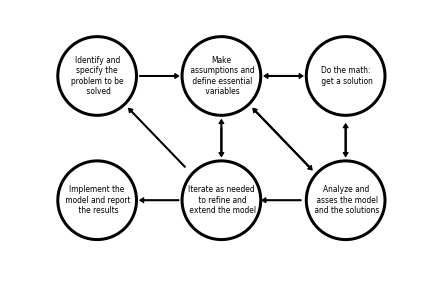
\includegraphics{fig-modeling-process}}
	\end{figure}
\end{frame}
%-------------------------------------------------------------------------------
%-------------------------------------------------------------------------------
%-------------------------------------------------------------------------------
%-------------------------------------------------------------------------------
\begin{frame}\textbf{Famous examples}\vspace{0.3cm}

\begin{itemize}\setlength\itemsep{1em}
\item \textbf{Lemons model \cite{Akerlof.1970}}, market unraveling in presence of asymmetric information
\item \textbf{Roy model \cite{Roy.1951}}, static model of self-selection and comparative advantage
\item \textbf{Career decisions model \cite{Keane.1997}}, dynamic model human capital investment with schooling and on-the-job training
\item $\hdots$
\end{itemize}

\end{frame}
